\documentclass{beamer}

\mode<presentation>
{
  \usetheme{classic}
  \setbeamercovered{transparent}
}

\usepackage[english]{babel}
\usepackage[latin1]{inputenc}
\usepackage{times}
\usepackage[T1]{fontenc}
\usepackage{url}

\title[CLS]{Common Lisp Statistics}
\subtitle{Using History to design better data analysis environments}
\author[Rossini]{Anthony~(Tony)~Rossini}

\institute[Novartis and University of Washington]{
  Group Head, Modeling and Simulation Statistics\\
  Novartis Pharma AG, Switzerland
  \and
  Affiliate Assoc Prof, Biomedical and Health Informatics\\
  University of Washington, USA}

\date[Vanderbilt]{Vanderbilt, Sept 2009, Nashville USA}
\subject{Statistical Computing Environments}

\begin{document}

\begin{frame}
  \titlepage
\end{frame}

\begin{frame}[fragile]{Intro to Lisp notation}
\begin{verbatim}
;; This is a comment
#|
    and so is this
|#
'(a list of things to become data)
(list a list of things to become data)
(what-I-execute with-one-thing with-two-thing)
;; that is:
(my-fcn-name input1 
             input2) ; and to auto-gen input1:
(my-fcn-name (my-fcn-name input3 input4)
             input2)
\end{verbatim}
\end{frame}  


\begin{frame}{What do you do?}
When you begin to work on an activity (methodological, theoretical,
application/substantive), and go to the keyboard to work on a
computer, {\textbf what do you do?}
\end{frame}


\section{Computable Statistics}

\begin{frame}{Can we compute with them?}
  3 Toy Examples:
  \begin{itemize}
  \item Statistical Research (``Annals work'')
  \item Consulting, Applied Statistics, Scientific Honesty.
  \item Reimplementation.
  \end{itemize}
  Can ``compute'' with the information given?  (that is:
  \begin{itemize}
  \item do we have sufficient information to communicate enough for
    the right person to understand or recreate the effort?
  \item have we sufficient clarity to prevent misunderstandings about
    intentions and claims?
  \end{itemize}
  )
\end{frame}

\begin{frame}[fragile]{Example 1: Theory\ldots}
  \label{example1}
  Let $f(x;\theta)$ describe the likelihood of XX under the following
  assumptions.  
  \begin{enumerate}
  \item assumption-1
  \item assumption-2
  \end{enumerate}
  Then if we use the following algorithm:
  \begin{enumerate}
  \item step-1
  \item step-2
  \end{enumerate}
  then $\hat{\theta}$ should be $N(0,\hat\sigma^2)$ with the following
  characteristics\ldots
\end{frame}

\begin{frame}
  \frametitle{Can we compute, using this description?}
  Given the information at hand:
  \begin{itemize}
  \item we ought to have a framework for initial coding for the
    actual simulations (test-first!)
  \item the implementation is somewhat clear
  \item We should ask: what theorems have similar assumptions?
  \item We should ask: what theorems have similar conclusions but
    different assumptions?
  \end{itemize}
\end{frame}
\begin{frame}[fragile]{Realizing Theory}
\small{
\begin{verbatim}  
(define-theorem my-proposed-theorem
  (:theorem-type '(distribution-properties
                   frequentist likelihood))
  (:assumes '(assumption-1 assumption-2))
  (:likelihood-form
     (defun likelihood (data theta gamma)
       (exponential-family theta gamma)))
  (:compute-by
   '(progn
      (compute-start-values thetahat gammahat)
        (until (convergence)
          (setf convergence
                (or (step-1 thetahat)
                    (step-2 gammahat))))))
  (:claim (equal-distr '(thetahat gammahat) 'normal))))
\end{verbatim}
}
\end{frame}

\begin{frame}[fragile]{It would be nice to have}
\begin{verbatim}
   (theorem-veracity 'my-proposed-theorem)
\end{verbatim}
returning some indication of how well it met given computable claims,
modulo what proportion of computable claims could be tested.
\begin{itemize}
\item and have it run some illustrative simulations which suggest
  which might be problematic in real situations, and real situations
  for which there are no problems.
\item and work through some of the logic based on related claims using
  identical assumptions to confirm some of the results
\end{itemize}
\end{frame}

\begin{frame}[fragile]{and why not...?}
\begin{verbatim}
   (when (> (theorem-veracity
              'my-proposed-theorem)
            0.8)
      (make-draft-paper 'my-proposed-theorem
                        :style :JASA
                        :output-formats
                           '(LaTeX MSWord)))
\end{verbatim}
\end{frame}

\begin{frame}{Comments}
  \begin{itemize}
  \item Of course the general problem is very difficult, but one must
    start somewhere.
  \item I'm working on some basic statistical proof of concepts (not
    finished): T-Test, linear regression (LS-based, Normal-Normal Bayesian)
  \item Areas targetted for medium-term future: resampling methods and
    similar algorithms.
  \end{itemize}
\end{frame}

\begin{frame}
  \frametitle{Example 2: Practice\ldots} 
  \label{example2}
  The dataset comes from a series of clinical trials, some with active
  control and others using placebo control.  We model the primary
  endpoint, ``relief'', as a binary random variable.  There is a
  random trial effect on relief as well as severity due to differences
  in recruitment and inclusion/exclusion criteria from 2 different
  trial networks.
\end{frame}

\begin{frame}
  \frametitle{Can we compute, using this description?}
  \begin{itemize}
  \item With a real such description, it is clear what some of the
    potential models might be for this dataset
  \item It should be clear how to start thinking of a data dictionary
    for this problem.
  \end{itemize}
\end{frame}

\begin{frame}[fragile]{Can we compute?}
\begin{verbatim}
(dataset-metadata paper-1
  :context 'clinical-trial 'randomized 
     'active-ctrl 'placebo-ctrl 'metaanalysis
  :variables '((relief :model-type dependent
                       :distr binary)
               (trial :model-type independent
                      :distr categorical)
               (disease-severity))
  :metadata '(incl-crit-net1 excl-crit-net1
              incl-crit-net1 excl-crit-net2
              recr-rate-net1 recr-rate-net2))
  (propose-analysis paper-1)
    ; => (list 'tables '(logistic-regression))
\end{verbatim}
\end{frame}

\begin{frame}{Example 3: The Round-trip\ldots} 
  \label{example3}
  The first examples describe ``ideas $\rightarrow$ code''

  Consider the last time you read someone else's implementation of a
  statistical procedure (i.e. R package code).  When you read the
  code, could you see:
  \begin{itemize}
  \item the assumptions used?
  \item the algorithm implemented?
  \item practical guidance for when you might select the algorithm
    over others? 
  \item practical guidance for when you might select the
    implementation over others? 
  \end{itemize}
  These are usually components of any reasonable journal article.
  \textit{(Q: have you actually read an R package that wasn't yours?)}
\end{frame}

\begin{frame}{Exercise left to the reader!}

%   (aside: I have been looking at the \textbf{stats} and \textbf{lme4}
%   packages recently -- \textit{for me}, very clear numerically, much
%   less so statistically)
\end{frame}

\section{Context}

\begin{frame}{Point of Examples}
  \begin{itemize}
  \item Few statistical concepts are ``computable'' with existing systems.

  \item Some of this work is computable, let the computer do it.

  \item There is little point in having people re-do basics

  \item Computing environments for statistical work have been stable
    for far too long, and limit the development and implementation of
    better, more efficient, and more appropriate methods by allowing
    people to be lazy (i.e. classic example of people publishing
    papers on changes which are very minimal from a
    methodological/theoretical view, but very difficult from an
    implementation/practical view).
  \end{itemize}
\end{frame}

\begin{frame}{Current State}

  The current approaches to how statisticians interface with computers
  to perform data analysis can be put into 2 camps
  \begin{enumerate}
  \item GUI with a spreadsheet (Excel/Minitab/Rcmdr without the
    script)
  \item applications programming (with
  \end{enumerate}
  There are different levels of sophistication, and some merging.
\end{frame}

\begin{frame}{Issues which arise when computing...}
  \begin{enumerate}
  \item relevant substantive issues (causality, variable independence,
    design issues such as sampling strategies) not incorporated.
  \item irrelevant substantive issues (coding, wide vs. long
    collection, other non-statistical data management issues) become
    statistically-relevant.
  \item little support for encoding theoretical considerations (``expert
    systems'' for guidance).  Must be hard-coded in and hard-coded
    away (``stars for p-values as evil'').   Nearly impossible to
    construct and apply philosophical opinions to ensure appropriate
    use (and training through use) of singular or personalized
    mixtures of statistical philosophies when doing data analysis (or
    methodological development, or theoretical development).
  \end{enumerate}
\end{frame}

\begin{frame}{Problem Statement}

  How can statistical computing environments support appropriate use
  of statistical concepts (algorithmic, knowledge-centric,
  knowledge-managing, philosophical discipline), so that the computing
  structure doesn't rely on data-munging or numerical skill?

\end{frame}


\begin{frame}{Goals for this Talk}{(define, strategic approach,
    justify)}

  \begin{itemize}
  \item To describe the concept of \alert{computable statistics},
    placing it in a historical context.

  \item To demonstrate that \alert{a research program}
    implemented through  simple steps can increase the efficiency  of
    statistical computing approaches by  clearly describing both:
    \begin{itemize}
    \item numerical characteristics of procedures,
    \item statistical concepts driving them.
    \end{itemize}

  \item To justify that the \alert{approach is worthwhile} and
    represents a staged effort towards \alert{increased use of best
      practices} and efficient tech transfer of modern statistical
    theory (i.e. why must we wait 10 years for Robins' estimation
    approaches?)
  \end{itemize}
  (unfortunately, the last is still incomplete)
\end{frame}

\section{CLS Works?}
\label{sec:work}

\begin{frame}{Is it Vaporware? Not quite}
  The follow is possible with the help of the open source Common Lisp
  community, who provided most of the packages, tools, and glue.
  (Tamas Papp, Raymond Toy, Mark Hoemmomem, and many, many others).
  Most of the underlying code was written by others, and ``composed''
  by me.
\end{frame}

\subsection{Graphics}
\label{sec:work:graphics}

\begin{frame}{Silly Visualization Example}
  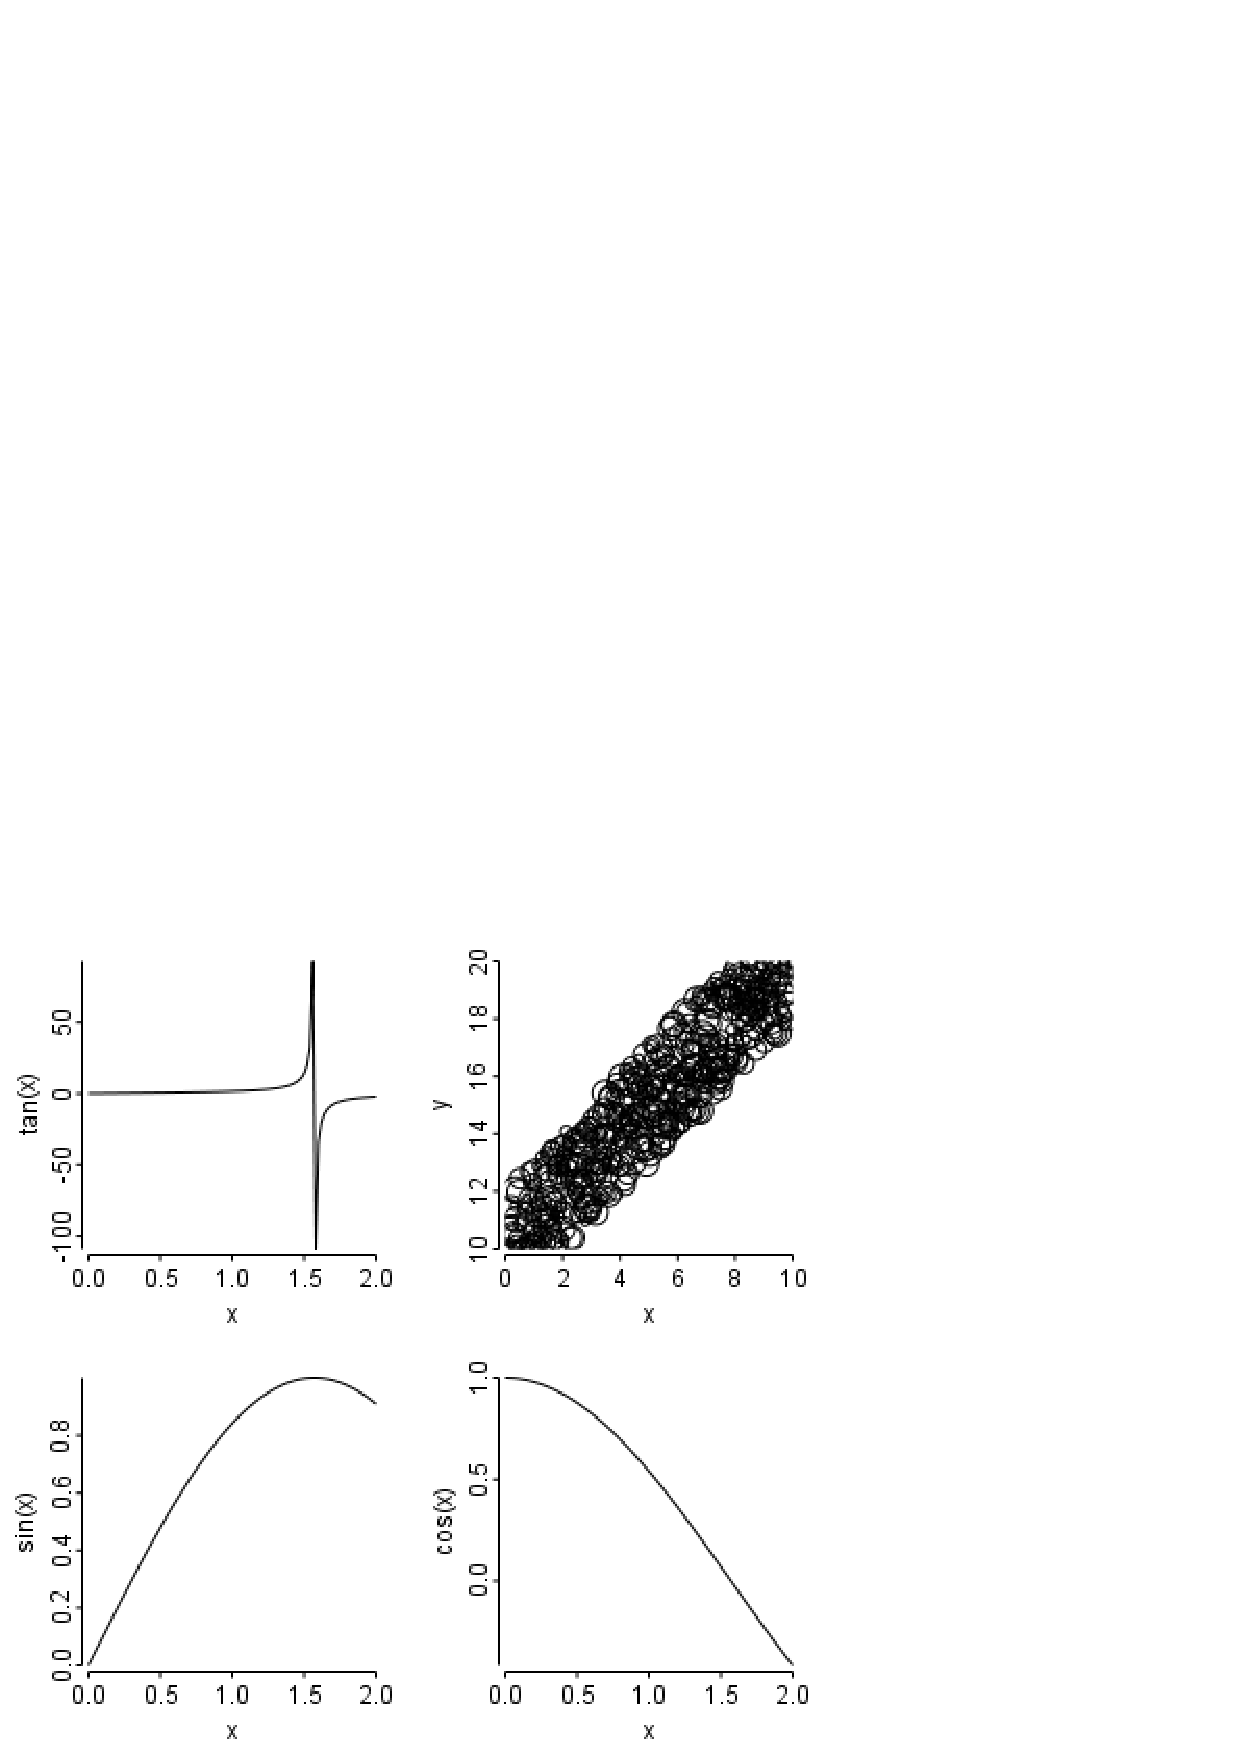
\includegraphics[width=3in,height=3in]{./test1.png}
\end{frame}

\begin{frame}[fragile]{How?}
\begin{verbatim}
(defparameter *frame2*
   (as-frame (create-xlib-image-context 200 200)
   	    :background-color +white+))
(bind ((#2A((f1 f2) (f3 f4))
       (split-frame *frame2*
                    (percent 50)
                    (percent 50))))
  (defparameter *f1* f1) ; lower left   
  (defparameter *f2* f2) ; lower right  f3  f4
  (defparameter *f3* f3) ; top left     f1  f2
  (defparameter *f4* f4)); top right
\end{verbatim}
\end{frame}

\begin{frame}[fragile]{Functions to Plot}
\begin{verbatim}
(plot-function *f1* #'sin
  (interval-of 0 2)
  :x-title "x" :y-title "sin(x)")
(plot-function *f2* #'cos (interval-of 0 2)
  :x-title "x" :y-title "cos(x)")
(plot-function *f3* #'tan (interval-of 0 2)
  :x-title "x" :y-title "tan(x)")
\end{verbatim}
\end{frame}

\begin{frame}[fragile]{Things to Plot}
\small{
\begin{verbatim}
(let* ((n 500)
       (xs (num-sequence
             :from 0 :to 10 :length n))
       (ys (map 'vector
              #'(lambda (x) (+ x 8 (random 4.0)))
              xs))
       (weights
          (replicate #'(lambda () (1+ (random 10)))
                     n 'fixnum))
       (da (plot-simple *f4*
             (interval-of 0 10)
             (interval-of 10 20)
             :x-title "x" :y-title "y")))
  (draw-symbols da xs ys :weights weights))
\end{verbatim}
}
\end{frame}

\begin{frame}[fragile]{Copying existing graphics}
  And we generated the figure on the first page by:
\begin{verbatim}
(xlib-image-context-to-png
   (context *f1*)
   "/home/tony/test1.png")
\end{verbatim}
\end{frame}

\subsection{Statistical Models}
\label{sec:work:statmod}

\begin{frame}[fragile]{Linear Regression}
\small{
\begin{verbatim}
;; Worse than LispStat, wrapping LAPACK's dgelsy:
(defparameter *result1*
   (lm (list->vector-like iron)
       (list->vector-like absorbtion)))
*result*1 =>
((#<LA-SIMPLE-VECTOR-DOUBLE (2 x 1)
 -11.504913191235342
 0.23525771181009483>
  2)

 #<LA-SIMPLE-MATRIX-DOUBLE  2 x 2
 9.730392177126686e-6 -0.001513787114206932
 -0.001513787114206932 0.30357851215706255>   

 13 2)
\end{verbatim}
}
\end{frame}

\subsection{Data Manip/Mgmt}
\label{sec:work:data}

\begin{frame}[fragile]{DataFrames}
\small{
\begin{verbatim}
(defparameter *my-df-1*
  (make-instance 'dataframe-array
	 :storage #2A((1 2 3 4 5) (10 20 30 40 50))
	 :doc "This is a boring dataframe-array"
	 :case-labels (list "x" "y")
	 :var-labels (list "a" "b" "c" "d" "e")))

(xref *my-df-1* 0 0) ; API change in progress

(setf (xref *my-df-1* 0 0) -1d0)
\end{verbatim}
}
\end{frame}

\begin{frame}[fragile]{Numerical Matrices}
\small{
\begin{verbatim}
(defparameter *mat-1*
  (make-matrix 3 3
     :initial-contents #2A((2d0 3d0 -4d0)
                           (3d0 2d0 -4d0)
                           (4d0 4d0 -5d0))))

(xref *mat-1* 2 0) ; => 4d0  ; API change
(setf (xref *mat-1* 2 0) -4d0) 

(defparameter *xv*
 (make-vector 4 :type :row 
   :initial-contents '((1d0 3d0 2d0 4d0))))
\end{verbatim}
}
\end{frame}

\begin{frame}[fragile]{Macros make the above tolerable}
\begin{verbatim}
(defparameter *xv*
 (make-vector 4 :type :row 
   :initial-contents '((1d0 3d0 2d0 4d0))))

; can use defmacro for the following syntax =>

(make-row-vector *xv* '((1d0 3d0 2d0 4d0)))

; or reader macros for the following:
#mrv(*xv* '((1d0 3d0 2d0 4d0)))
\end{verbatim}
\end{frame}

\section{Common Lisp Statistics}
\label{sec:CLS}

\begin{frame}{Why CLS?}
  \begin{itemize}
  \item a component-based structure for statistical computing,
    allowing for small and specific specification.
  \item a means to drive philosophically customized data analysis, and
    enforce a structure to allow simple comparisons between
    methodologies.
  \item This is a ``customization'' through packages to support
    statistical computing, not a independent language.  ``Ala Carte'',
    not ``Menu''.
  \end{itemize}
\end{frame}

\subsection{Implementation Plans}
\label{sec:CLS:impl}


\begin{frame}{Current Functionality}
  \begin{itemize}
  \item basic dataframes (similar to R); subsetting API under
    development.
  \item Basic regression (similar to XLispStat)
  \item matrix storage both in foreign and lisp-centric areas.
  \item LAPACK (small percentage, increasing), working with both
    matrix storage types
  \item static graphics (X11) including preliminary grid functionality based
    on CAIRO.  Generation of PNG files from graphics windows.
  \item CSV file support
  \item Common Lisp!
  \end{itemize}
\end{frame}

\begin{frame}[fragile]{Computational Environment Supported}
  \begin{itemize}
  \item works on Linux, with recent SBCL versions
  \item Definitely works on bleeding edge Debian (unstable).
  \item Has worked for weak definitions of ``work'' on 4 different
    people's computers (not quite, but sort of requires a
    \verb+/home/tony/+ !)
  \end{itemize}
\end{frame}

\begin{frame}{Goals}
  Short Term
  \begin{itemize}
  \item Better integration of data structures with statistical routines
    (auto-handling with dataframes, rather than manual parsing). 
  \item dataframe to model-matrix tools (leveraging old XlispStat GEE
    package)
  \end{itemize}
  Medium/Long Term 
  \begin{itemize}
  \item Support for other Common Lisps
  \item Cleaner front-end API to matrices and numerical algorithms
  \item constraint system for different statistical algorithm
    development, as well as for interactive GUIs and graphics
  \item LispStat compatible (object system in-progress, GUI to do)
  \item Integrated invisible parallelization when more efficient
    (multicore, threading, and user-space systems)
  \end{itemize}
\end{frame}


\section{Vaporware?}

\begin{frame}[fragile]{What does NOT work?}
  Primarily, the reason that we doing this:
  
  \textbf{Computable and Executable Statistics}

  but consider XML:
\begin{verbatim}
<car brand="honda" engine="4cyl">accord</car>
\end{verbatim}
becomes
\begin{verbatim}
; data follows keywords...
(car :brand 'honda :engine "4cyl" accord)
\end{verbatim}
\end{frame}

\section{Discussion}




\begin{frame}{Why use Common Lisp?}
  \begin{itemize}
  \item Parens provide clear delineation of a \textbf{Complete
      Thought} (functional programming with side effects).
  \item Lisp-2 (symbols represent a different function and variable)
  \item ANSI standard (built by committee, but the committee was
    reasonably smart)
  \item Many implementations
  \item Most implementations are interactive \textbf{compiled}
    languages (few are interpreted, nearly all  byte-compiled).
  \item The Original \emph{Programming with Data} Language
    (\emph{Programs are Data} and \emph{Data are Executable} apply).
  \item advanced, powerful, first-class macros (macros functionally
    re-write code, allowing for structural clarity and complete
    destruction of syntax, should that be reasonable)
  \end{itemize}
\end{frame}

\begin{frame}{Available Common Lisp Packages}
  (They are packages and called packages, not libraries.  Some people
  can rejoice!)
  \begin{itemize}
  \item infrastructure \emph{enhancements}: infix-notation, data
    structures, control and flow structures
  \item numerics, graphics, GUIs, 
  \item primitive R to CL compiler (which could also be considered an
    object-code compiler for R); 3 interfaces which embed R within CL.
  \item Web 2.0 support and TeX-like reporting facilities for PDF
    output.
  \end{itemize}
  See \url{http://www.common-lisp.net/} and
  \url{http://www.cliki.org/}.  CLS sources can be found on
  \url{http://github.com/blindglobe/}
\end{frame}

\begin{frame}{Why not use R?}
  \begin{itemize}
  \item the R programming language is incomplete and under constant
    redefinition.  Common Lisp is standardized (for many years), with
    many implementations
  \item R isn't compiled and appliction delivery can be tough (package
    delivery is mostly solved)
  \item Without parens, Common Lisp could be R (interactive, or batch,
    or through ``compiled applications'').
  \item R is the Microsoft of statistical computing.
  \item many ``warts'' that R has, can't be fixed due to sizeable user
    populations or heavy-weight vested interests.
  \item Evolutionary development requires strawmen upon which to use
    for development.
\end{itemize}

\end{frame}

\begin{frame}{Conclusion}

  This slowly developing research program aims to a statistical
  computing system which enables sophisticated statistical research
  which can be readily transfer to applications, is supportable.

  Related numerical/statistical projects:
  \begin{itemize}
  \item Incanter : R/LispStat/Omegahat-like system for Clojure (Lisp
    on the JVM)
  \item FEMLisp : system/workshop for finite-element analysis modeling
    using Lisp
  \item matlisp/LispLab : LAPACK-based numerical linear algebra packages
  \item GSLL : GNU Scientific Library, Lisp interface.
  \item RCL, RCLG, CLSR (embedding R within Common Lisp)
  \end{itemize}
\end{frame}

\begin{frame}{What can you do to follow up?}

  \begin{itemize}
  \item Read:  Introduction to Common Lisp: Paul Graham's ANSI Common Lisp,
    enjoyable book with boring title, best intro to S4 classes
    around.  Practical Common Lisp, by Peter Seibel
  \item Consider:  how a computing environment could better support
    features in the research you do (event-time data, design,
    longitudinal data modeling, missing and coarsened data, multiple
    comparisons, feature selection). 
  \end{itemize}
  The next stage of reproducible research will require computable
  statistics (code that explains itself and can be parsed to generate
  knowledge about its claims; ``XML's promise'').
\end{frame}

\end{document}

%%%%%%%%%%%%%%%%%%%%%%%%%%%%%%%%%%%%%%%%%%%%%%%%%%%%%%%%%%%



\section{BACKUPS}


\section{Common Lisp}

\begin{frame}[fragile]{Finding out things}
  \begin{itemize}
  \item CL-NUMLIB
     num-sequence :from LOW to: HIGH :length SEQ-LENGTH 
     seq(from,to,by/length)
   \item
\begin{verbatim}
(documentation
     'cl-numlib:num-sequence
     'function)
\end{verbatim}
   \item This
  \end{itemize}
\end{frame}


\begin{frame}{Historical Computing Languages}
  \begin{itemize}
  \item FORTRAN : FORmula TRANslator.  Original numerical computing
    language, designed for clean implementation of numerical
    algorithms
  \item LISP : LISt Processor.  Associated with symbolic
    manipulation, AI, and knowledge approaches
  \end{itemize}

  They represent the 2 generalized needs of statistical computing,
  which could be summarized as
  \begin{itemize}
  \item algorithms/numerics,
  \item elicitation, communication, and generation of knowledge (``data
    analysis'')
  \end{itemize}
\end{frame}

\begin{frame}{Statistical Computing Environments}

  Past: 
  \begin{itemize}
  \item SPSS / BMDP / SAS
  \item S ( S, S-PLUS, R)
  \item LispStat ( XLispStat,  ViSta, ARC , CommonLispStat ) ; QUAIL
  \item XGobi (Orca / GGobi / Statistical Reality Engine)
  \item MiniTab
  \item Stata
  \item DataDesk
  \item Augsburg Impressionist series (MANET, 
  \item Excel
  \end{itemize}
  many others...

\end{frame}

\begin{frame}{How many are left?}

  \begin{itemize}
  \item R 
  \item SAS
  \item SPSS
  \item Stata
  \item Minitab
  \item very few others...    
  \end{itemize}
  ``R is the Microsoft of the statistical computing world'' -- anonymous.
\end{frame}

\begin{frame}{Selection Pressure}
  \begin{itemize}
  \item the R user population is growing rapidly, fueled by critical
    mass, quality, and value
  \item R is a great system for applied data analysis
  \item R is not such a great system for research into statistical
    computing (backwards compatibility, inertia due to user population)
  \end{itemize}
  There is a need for alternative experiments for developing new
  approaches/ideas/concepts. 
\end{frame}

\begin{frame}{Philosophically, why Common Lisp?}
  Philosophically:
  \begin{itemize}
  \item Lisp can cleanly present computational intentions, both
    symbolically and numerically.
  \item Semantics and context are important: well supported by Lisp
    paradigms.
  \item Lisp's parentheses describe singular, multi-scale,
    \alert{complete thoughts}.
  \end{itemize}

\end{frame}

\begin{frame}{Technically, why Common Lisp?}
  \begin{itemize}
  \item interactive COMPILED language (``R with a compiler'')
  \item CLOS is R's S4 object system ``done right''.
  \item clean semantics: modality, typing, can be expressed the way
    one wants it.
  \item programs are data, data are programs, leading to
  \item Most modern computing tools available (XML, WWW technologies)
  \item ``executable XML''
  \end{itemize}
  Common Lisp is very close in usage to how people currently use R
  (mostly interactive, some batch, and a wish for compilation efficiency).
\end{frame}

\subsection{Background}

\begin{frame}
  \frametitle{Desire: Semantics and Statistics}
  \begin{itemize}
  \item The semantic web (content which is self-descriptive) is an
    interesting and potentially useful idea.
    
  \item 
    Biological informatics support (GO, Entrez) has allowed for
    precise definitions of concepts in biology.

  \item It is a shame that a field like statistics, requiring such
    precision, has less than an imprecise and temporally instable
    field such as biology\ldots
  \end{itemize}

  How can we express statistical work (research, applied work) which
  is both human and computer readable (perhaps subject to
  transformations first)?
\end{frame}


% \subsection{Context}

% \begin{frame}{Context}{(where I'm coming from, my ``priors'')}
%   \begin{itemize}
%   \item Pharmaceutical Industry
%   \item Modeling and Simulation uses mathematical models/constructs to
%     record beliefs (biology, pharmacology, clinical science) for
%     explication, clinical team alignment, decision support, and
%     quality.
%   \item My work at Novartis is at the intersection of biomedical
%     informatics, statistics, and mathematical modeling.
%   \item As manager: I need a mix of applications and novel research development to
%     solve our challenges better, faster, more efficiently.
%   \item Data analysis is a specialized approach to computer
%     programming, \alert{different} than applications programming or
%     systems programming.
%   \end{itemize}
% \end{frame}


\subsection{Literate Programming is insufficient}

\begin{frame}{Literate Statistical Practice.}
  \begin{enumerate}
  \item Literate Programming applied to data analysis (Rossini, 1997/2001)
  \item among the \alert{most annoying} techniques to integrate into
    work-flow if one is not perfectly methodological.
  \item Some tools:
    \begin{itemize}
    \item ESS: supports interactive creation of literate programs.
    \item Sweave: tool which exemplifies reporting context; odfWeave
      primarily simplifies reporting.
    \item Roxygen: primarily supports a literate programming
      documentation style, not a literate data analysis programming
      style. 
  \end{itemize}
  \item ROI demonstrated in specialized cases: BioConductor.
  \item \alert{usually done after the fact} (final step of work-flow)
    as a documentation/computational reproducibility technique, rarely
    integrated into work-flow.
  \end{enumerate}
  Many contributors:
  Knuth, Claerbout, Carey, de Leeuw, Leisch, Gentleman, Temple-Lang,
  \ldots{}
\end{frame}

\begin{frame}
  \frametitle{Literate Programming}
  \framesubtitle{Why isn't it enough for Data Analysis?}

  Only 2 contexts: (executable) code and documentation.  Fine for
  application programming,  but for data analysis, we could benefit
  from:
  \begin{itemize}
  \item classification of statistical procedures
  \item descriptions of assumptions
  \item pragmatic recommendations
  \item inheritance of structure through the work-flow of a
    statistical methodology or data analysis project
  \item datasets and metadata
  \end{itemize}
  Concept: ontologies describing mathematical assumptions, applications
  of methods, work-flow, and statistical data structures can enable
  machine communication.
  
  (i.e. informatics framework ala biology)
\end{frame}


\begin{frame}{Communication in Statistical Practice}{\ldots is essential for \ldots}
  \begin{itemize}
  \item finding
  \item explanations
  \item agreement
  \item receiving information
  \end{itemize}
  \alert{``machine-readable'' communication/computation lets the
    computer help} \\
  Semantic Web is about ``machine-enabled computability''.
\end{frame}

\begin{frame}  \frametitle{Semantics}
  \framesubtitle{One definition: description and context}

  Interoperability is the key, with respect to
  \begin{itemize}
  \item ``Finding things''
  \item Applications and activities with related functionality
    \begin{itemize}
    \item moving information from one state to another (paper, journal
      article, computer program)
    \item computer programs which implement solutions to similar tasks
    \end{itemize}
  \end{itemize}
\end{frame}


\begin{frame}{Statistical Practice is somewhat restricted}
  {...but in a good sense, enabling potential for semantics...}

  There is a restrictable set of intended actions for what can be done
  -- the critical goal is to be able to make a difference by
  accelerating activities that should be ``computable'':
  \begin{itemize}
  \item restricted natural language processing
  \item mathematical translation
  \item common description of activities for simpler programming/data
    analysis (S approach to objects and methods)
  \end{itemize}
  R is a good basic start (model formulation approach, simple
  ``programming with data'' paradigm); we should see if we can do
  better!
\end{frame}

\begin{frame}{Computable and Executable Statistics requires}

  \begin{itemize}
  \item approaches to describe data and metadata (``data'')
    \begin{itemize}
    \item semantic WWW
    \item metadata management and integration, driving
    \item data integration
    \end{itemize}
  \item approaches to describe data analysis methods (``models'')
    \begin{itemize}
    \item quantitatively: many ontologies (AMS, etc), few meeting
      statistical needs.
    \item many substantive fields have implementations
      (bioinformatics, etc) but not well focused.
    \end{itemize}
  \item approaches to describe the specific form of interaction
    (``instances of models'')
    \begin{itemize}
    \item Original idea behind ``Literate Statistical Analysis''.
    \item That idea is suboptimal, more structure needed (not
      necessarily built upon existing...).
    \end{itemize}
  \end{itemize}
\end{frame}

\subsection{Common Lisp Statistics}

\begin{frame}
  \frametitle{Interactive Programming}
  \framesubtitle{Everything goes back to being Lisp-like}
  \begin{itemize}
  \item Interactive programming (as originating with Lisp): works
    extremely well for data analysis (Lisp being the original
    ``programming with data'' language).
  \item Theories/methods for how to do this are reflected in styles
    for using R.
  \end{itemize}
\end{frame}
 
\begin{frame}[fragile]
  \frametitle{Lisp}

  Lisp (LISt Processor) is different than most high-level computing
  languages, and is very old (1956).  Lisp is built on lists of things
  which are evaluatable.
\begin{verbatim}
(functionName data1 data2 data3)
\end{verbatim}
  or ``quoted'':
\begin{verbatim}
'(functionName data1 data2 data3)
\end{verbatim}
  which is shorthand for 
\begin{verbatim}
(list functionName data1 data2 data3)
\end{verbatim}
  The difference is important -- lists of data (the second/third) are
  not (yet?!) functions applied to (unencapsulated lists of) data (the first).
\end{frame}

\begin{frame}
  \frametitle{Features}
  \begin{itemize}
  \item Data and Functions semantically the same
  \item Natural interactive use through functional programming with
    side effects
  \item Batch is a simplification of interactive -- not a special mode!
  \end{itemize}
\end{frame}



\begin{frame}[fragile]{Representation: XML and Lisp}{executing your data}
  Many people are familiar with XML: 
\begin{verbatim}
<name phone="+41793674557">Tony Rossini</name>
\end{verbatim}
  which is shorter in Lisp:
\begin{verbatim}
(name "Tony Rossini" :phone "+41613674557")
\end{verbatim}
  \begin{itemize}
  \item Lisp ``parens'', universally hated by unbelievers, are
    wonderful for denoting when a ``concept is complete''.
  \item Why can't your data self-execute?
  \end{itemize}
\end{frame}

\begin{frame}[fragile]{Numerics with Lisp}
  \begin{itemize}
  \item addition of rational numbers and arithmetic
  \item example for mean
\begin{verbatim}
 (defun mean (x)
    (checktype x 'vector-like)
    (/ (loop for i from 0 to (- (nelts *x*) 1)
	  summing (vref *x* i))
       (nelts *x*)))
\end{verbatim}
  \item example for variance
\begin{verbatim}
(defun variance (x)
  (let ((meanx (mean x))
	(nm1 (1- (nelts x))))
     (/ (loop for i from 0 to nm1
	   summing (power (- (vref *x* i) meanx) 2)
        nm1))))
\end{verbatim}
  \item But through macros, \verb+(vref *x* i)+ could be
    \verb+#V(X[i])+ or your favorite syntax.
  \end{itemize}
  
\end{frame}


\begin{frame}{Common Lisp Statistics 1}
  \begin{itemize}
  \item Originally based on LispStat (reusability)
  \item Re-factored structure (some numerics worked with a 1990-era code base). 
  \item Current activities:
    \begin{enumerate}
    \item numerics redone using CFFI-based BLAS/LAPLACK (cl-blapack)
    \item matrix interface based on MatLisp
    \item starting design of a user interface system (interfaces,
      visuals).
    \item general framework for model specification (regression,
      likelihood, ODEs)
    \item general framework for algorithm specification (bootstrap,
      MLE, algorithmic data anaylsis methods).
    \end{enumerate}
  \end{itemize}
\end{frame}

\begin{frame}{Common Lisp Statistics 2}

  \begin{itemize}
  \item Implemented using SBCL.  Contributed fixes for
    Clozure/OpenMCL. Goal to target CLISP
  \item Supports LispStat prototype object system
  \item Package-based design -- only use the components you need, or
    the components whose API you like.
  \end{itemize}
\end{frame}

\section{Discussion}

\begin{frame}
  \frametitle{Outlook}
  \begin{itemize}
  \item Semantics and Computability have captured a great deal of
    attention in the informatics and business computing R\&D worlds
  \item Statistically-driven Decision Making and Knowledge Discovery
    is, with high likelihood, the next challenging stage after data
    integration.
  \item Statistical practice (theory and application) can be enhanced,
    made more efficient, providing  increased benefit to organizations
    and groups using appropriate methods.
  \item Lisp as a language, shares characteristics of both Latin
    (difficult dead language useful for classical training) and German
    (difficult living language useful for general life).  Of course,
    for some people, they are not difficult.
  \end{itemize}

\end{frame}

\begin{frame}
  The research program described in this talk is currently driving the
  design of CommonLisp Stat, which leverages concepts and approaches
  from the dead and moribund LispStat project.

  \begin{itemize}
  \item \url{http://repo.or.cz/w/CommonLispStat.git/}
  \item \url{http://www.github.com/blindglobe/}
  \end{itemize}

\end{frame}
\begin{frame}{Final Comment}

  \begin{itemize}
  \item In the Pharma industry, it is all about getting the right
    drugs to the patient faster.  Data analysis systems seriously
    impact this process, being potentially an impediment or an
    accelerator.

    \begin{itemize}
    \item \alert{Information technologies can increase the efficiency
        of statistical practice}, though innovation change management
      must be taking into account.  (i.e. Statistical practice, while
      considered by some an ``art form'', can benefit from
      industrialization).
    \item \alert{Lisp's features match the basic requirements we need}
      (dichotomy: programs as data, data as programs).  Sales pitch,
      though...
    \item Outlook: Lots of work and experimentation to do!
    \end{itemize}
  \end{itemize}
\end{frame}


% % All of the following is optional and typically not needed. 
% \appendix


% \section<presentation>*{\appendixname}


% \begin{frame} \frametitle{Complements and Backup}
%   No more, stop here.  Questions?  (now or later).
% \end{frame}

% \begin{frame}{The Industrial Challenge.}{Getting the Consulting Right.}
%   % - A title should summarize the slide in an understandable fashion
%   %   for anyone how does not follow everything on the slide itself.

%   \begin{itemize}
%   \item Recording assumptions for the next data analyst, reviewer.
%     Use \texttt{itemize} a lot.
%   \item
%     Use very short sentences or short phrases.
%   \end{itemize}
% \end{frame}


% \begin{frame}{The Industrial Challenge.}{Getting the Right Research Fast.}
%   % - A title should summarize the slide in an understandable fashion
%   %   for anyone how does not follow everything on the slide itself.

%   \begin{itemize}
%   \item
%     Use \texttt{itemize} a lot.
%   \item
%     Use very short sentences or short phrases.
%   \end{itemize}
% \end{frame}


% \begin{frame}{Explicating the Work-flow}{QA/QC-based improvements.}


% \end{frame}

% \section{Motivation}

% \subsection{IT Can Speed up Deliverables in Statistical Practice}

% \begin{frame}{Our Generic Work-flow and Life-cycle}
%   {describing most data analytic activities}
%   Workflow:
%   \begin{enumerate}
%   \item Scope out the problem
%   \item Sketch out a potential solution
%   \item Implement until road-blocks appear
%   \item Deliver results 
%   \end{enumerate}

%   Lifecycle:
%   \begin{enumerate}
%   \item paper sketch
%   \item 1st e-draft of text/code/date (iterate to \#1, discarding)
%   \item cycle through work
%   \item publish
%   \item ``throw-away''
%   \end{enumerate}
%   but there is valuble information that could enable the next
%   generation!
% \end{frame}

% \begin{frame}[fragile]{Paper $\rightarrow$ Computer  $\rightarrow$ Article $\rightarrow$ Computer}{Cut and Paste makes for large errors.}
%   \begin{itemize}
%   \item Problems in a regulatory setting
%   \item Regulatory issues are just ``best practices''
%   \end{itemize}

%   Why do we ``copy/paste'', or analogously, restart our work?

%   pro:
%   \begin{itemize}
%   \item every time we repeat, we reinforce the idea in our brain
%   \item review of ideas can help improve them
%   \end{itemize}
%   con:
%   \begin{itemize}
%   \item inefficiency
%   \item introduction of mistakes
%   \item loss of historical context
%   \item changes to earlier work (on a different development branch)
%     can not propagate. 
%   \end{itemize}
% \end{frame}

% \section{Semantics and Statistical Practice}


% \begin{frame}
%   \frametitle{Statistical Activity Leads to Reports}
%   \framesubtitle{You read what you know, do you understand it?}

%   How can we improve the communication of the ideas we have?

%   Precision of communication?

% \end{frame}



% \begin{frame}  \frametitle{Communication Requires Context}
%   \framesubtitle{Intentions imply more than one might like...}

%   \begin{itemize}
%   \item Consideration of what we might do
%   \item Applications with related functionality
%   \end{itemize}
% \end{frame}



% \begin{frame}
%   \frametitle{Design Patterns}
%   \framesubtitle{Supporting Work-flow Transitions}
  
%   (joint work with H Wickham): The point of this research program is
%   not to describe what to do at any particular stage of work, but to
%   encourage researchers and practitioners to consider how the
%   translation and transfer of information between stages so that work
%   is not lost.

%   Examples of stages in a work-flow:
%   \begin{itemize}
%   \item planning, execution, reporting;
%   \item scoping, illustrative examples or counter examples, algorithmic construction,
%     article writing.
%   \item descriptive statistics, preliminary inferential analysis,
%     model/assumption checking, final inferential analysis,
%     communication of scientific results
%   \end{itemize}
%   Description of work-flows is essential to initiating discussions on
%   quality/efficiency of approaches to work.
% \end{frame}

% \section{Design Challenges}

% \begin{frame}
%   \frametitle{Activities are enhanced by support}

%   \begin{itemize}
%   \item Mathematical manipulation can be enhanced by symbolic
%     computation
%   \item Statistical programming can be enabled by examples and related
%     algorithm implementation
%   \item Datasets, to a limited extent, can self-describe.
%   \end{itemize}
% \end{frame}

% \begin{frame}
%   \frametitle{Executable and Computable Science}
  
%   Use of algorithms and construction to describe how things work.

%   Support for agent-based approaches
% \end{frame}


% \begin{frame}
%   \frametitle{What is Data?  Metadata?}

%   Data: what we've observed

%   MetaData: context for observations, enables semantics.
% \end{frame}




% % \begin{frame}[fragile]
% %   \frametitle{Defining Variables}
% %   \framesubtitle{Setting variables}
% % \begin{verbatim}
% % (setq <variable> <value>)
% % \end{verbatim}
% %   Example:
% % \begin{verbatim}
% % (setq ess-source-directory
% %       "/home/rossini/R-src")
% % \end{verbatim}
% % \end{frame}

% % \begin{frame}[fragile]
% %   \frametitle{Defining on the fly}
% % \begin{verbatim}
% % (setq ess-source-directory
% %    (lambda () (file-name-as-directory
% %          (expand-file-name
% %            (concat (default-directory)
% %                    ess-suffix "-src")))))
% % \end{verbatim}
% %   (Lambda-expressions are anonymous functions, i.e. ``instant-functions'')
% % \end{frame}


% % \begin{frame}[fragile]
% %   \frametitle{Function Reuse}
% %   By naming the function, we could make the previous example reusable
% %   (if possible):
% % \begin{verbatim}
% % (defun my-src-directory ()
% %       (file-name-as-directory
% %          (expand-file-name
% %            (concat (default-directory)
% %                    ess-suffix "-src"))))
% % \end{verbatim}
% %   Example:
% % \begin{verbatim}
% % (setq ess-source-directory (my-src-directory))
% % \end{verbatim}
% % \end{frame}


% % \begin{frame}
% %   \frametitle{Equality Among Packages}
% %   \begin{itemize}
% %   \item more/less equal can be described specifically through
% %     overriding imports.
% %   \end{itemize}
% % \end{frame}


% \subsection<presentation>*{For Further Reading}

% \begin{frame}[allowframebreaks]
%   \frametitle<presentation>{Related Material}
    
%   \begin{thebibliography}{10}
    
%   \beamertemplatebookbibitems
%   % Start with overview books.

%   \bibitem{LispStat1990}
%     L.~Tierney
%     \newblock {\em LispStat}.
 
%   \beamertemplatearticlebibitems
%   % Followed by interesting articles. Keep the list short. 

%   \bibitem{Rossini2001}
%     AJ.~Rossini
%     \newblock Literate Statistical Practice
%     \newblock {\em Proceedings of the Conference on Distributed
%       Statistical Computing}, 2001.

%   \bibitem{RossiniLeisch2003}
%     AJ.~Rossini and F.~Leisch
%     \newblock Literate Statistical Practice
%     \newblock {\em Technical Report Series, University of Washington
%       Department of Biostatistics}, 2003.

%   \beamertemplatearrowbibitems
%   % Followed by interesting articles. Keep the list short. 

%   \bibitem{CLS}
%     Common Lisp Stat, 2008.
%     \newblock \url{http://repo.or.cz/CommonLispStat.git/}

%   \end{thebibliography}
% \end{frame}
